% Created 2026-05-11 Mon 12:33
% Intended LaTeX compiler: pdflatex
\documentclass[11pt]{article}

\usepackage[utf8]{inputenc}
\usepackage[T1]{fontenc}
\usepackage{graphicx}
\usepackage{longtable}
\usepackage{wrapfig}
\usepackage{rotating}
\usepackage[normalem]{ulem}
\usepackage{amsmath}
\usepackage{amssymb}
\usepackage{capt-of}
\usepackage{hyperref}
\usepackage{minted}
\author{flavio}
\date{\today}
\title{\#+title: UML}
\hypersetup{
 pdfauthor={flavio},
 pdftitle={\#+title: UML},
 pdfkeywords={},
 pdfsubject={},
 pdfcreator={},
 pdflang={English}}
\begin{document}

\maketitle
\tableofcontents

\section{UML}
\label{sec:org290821d}
\emph{Unified} \emph{Modeling} \emph{Language}.  Un linguaggio di modellazione e di specifica basato sul paradigma agli oggetti. Un linguaggio che permette di disegnare in maniera standard, unficato e quindi universalmente comprensibile diversi diagrammi.
\subsection{Object oriented analysis}
\label{sec:orgcad9dbe}
Delle figure della compagnia esperte di Object Oriented analysis cercano di capire il dominio che il nostro cliente chiede di analizzare: prende consapevolezza degli oggetti nel mondo reale e identifica le identità.
\subsubsection{Fasi object Analysis}
\label{sec:org5cc6096}
\begin{enumerate}
\item Identificare le entità
\begin{enumerate}
\item Modellare le entità in uml
\begin{enumerate}
\item Creazione delle classi in java
\begin{enumerate}
\item Creazione dell'applicazione in java
\end{enumerate}
\end{enumerate}
\end{enumerate}
\end{enumerate}
\subsection{Basi del linguaggio}
\label{sec:orgad1efe5}
Ciò che studieremo saranno i diagrammi delle classi. I diagrammi delle classi si compongono di package di classi che possono contenere classi o a loro volta altri package detti subpackage. Ogni package è una cartella che contiene classi (file).
\subsubsection{diagramma UML}
\label{sec:org35e3158}
\begin{center}
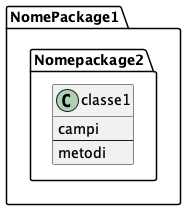
\includegraphics[width=.9\linewidth]{test3.png}
\label{}
\end{center}

prendiamo per esempio la classe Rettangolo in Java

\begin{minted}[]{java}
class Rettangolo{
    private double x,y,lunghezza;
    private double altezza;

    public Rettangolo(double x, double y, double lunghezza)
        {
            this.x = x;
            this.y = y;
            this.lunghezza = lunghezza;
        }
    public void trasla(double x, double y)
        {
            this.x = x;
            this.y = y;
        }
    public String toString()
        {
            double x2 = x + lunghezza;
            double y2 = y + lunghezza;
            return "("+x+","+y+")" +"("+x2+","+"y2"+")";
        }
}
\end{minted}
in uml:
\begin{center}
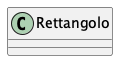
\includegraphics[width=.9\linewidth]{rettnagolo_uml.png}
\label{}
\end{center}
\subsubsection{Visibilità}
\label{sec:org8855d2b}
\texttt{+} visibilità pubblica: Ogni elemento che può accedere alla classe può anche accedere a ogni suo membro con visibilità pubblica
\texttt{-} Visibilità privata: solo le operazioni della classe possono accedere ai membri della classe.
\texttt{\#} Visibilità protetta: solo le operazioni della classe e delle sue sottoclassi possono accedere alla classe.
\texttt{\textasciitilde{}} Visibilità package: ogni elemento nelo stesso package della classe (o suo sottopackage annidato) può accedere ai membri della classe con visibilità package.
\end{document}
